\documentclass[aspectratio=169,10pt]{beamer}

\usepackage[T1]{fontenc}
\usepackage{amsmath}
\usepackage{amssymb}
\usepackage{amsthm}
\usepackage{bm}
\usepackage{graphicx}
\usepackage{subcaption}
\usepackage{booktabs}
\usepackage{xcolor}
\usepackage{listings}
\usepackage{hyperref}
\usepackage{lmodern}
\usepackage{cancel}
\usepackage{tikz}
\usetikzlibrary{positioning}
\usetikzlibrary{calc}
\usetikzlibrary{decorations.markings}
\usepackage{tikz-feynman}
\tikzfeynmanset{compat=1.1.0}
\usepackage{pgfplots}
\pgfplotsset{compat=1.18}

% comandi
\newcommand{\Lag}{\mathcal{L}}
\newcommand{\p}{\partial}
\newcommand{\bepsilon}{\bar{\epsilon}}
\newcommand{\MMS}{\overline{\mathrm{MS}}}
\usepackage{xparse}
\usepackage{appendixnumberbeamer}

\NewDocumentCommand{\supcite}{o m}{%
  \textsuperscript{\scriptsize%
    \IfNoValueTF{#1}{\cite{#2}}{\cite[#1]{#2}}%
  }%
}

% diagrammi
\newcommand{\ScalarPropagator}{%
\begin{tikzpicture}[scale=0.7, transform shape, baseline={([yshift=-0.1cm]current bounding box.center)}]
    \begin{feynman}
        \vertex (i) at (-1.5,0);
        \vertex (f) at (1.5,0);
        
        \diagram*{(i) -- [scalar] (f)};
        
    \end{feynman}
\end{tikzpicture}%
}

\newcommand{\ScalarPropagatorCounterterm}[1]{%
\begin{tikzpicture}[scale=0.7, transform shape, baseline={([yshift=-0.25cm]current bounding box.center)}]
    \begin{feynman}
        \vertex (i) at (-1.5,0);
        \vertex (f) at (1.5,0);
        \vertex [crossed dot] (v) at (0,0) {};
        
        \diagram*{(i) -- [scalar] (v) -- [scalar] (f)};

        \node at (0.4,0.3) {$#1$};
    \end{feynman}
\end{tikzpicture}%
}

\newcommand{\FourScalarVertex}{%
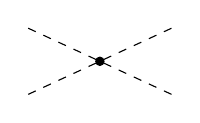
\begin{tikzpicture}[scale=0.7, transform shape, baseline={([yshift=-0.1cm]current bounding box.center)}]
    \begin{feynman}
        \vertex (i1) at (-1.3,0.6);
        \vertex (i2) at (-1.3,-0.6);
        \vertex [dot] (v) at (0,0) {};
        \vertex (f1) at (1.3,0.6);
        \vertex (f2) at (1.3,-0.6);

        \diagram*{(i1) -- [scalar] (v), (i2) -- [scalar] (v), (v) -- [scalar] (f1), (v) -- [scalar] (f2)};
        
    \end{feynman}
\end{tikzpicture}%
}

\newcommand{\FourScalarVertexCounterterm}[1]{%
\begin{tikzpicture}[scale=0.7, transform shape, baseline={([yshift=-0.1cm]current bounding box.center)}]
    \begin{feynman}
        \vertex (i1) at (-1.3,0.6);
        \vertex (i2) at (-1.3,-0.6);
        \vertex [crossed dot] (v) at (0,0) {};
        \vertex (f1) at (1.3,0.6);
        \vertex (f2) at (1.3,-0.6);

        \diagram*{(i1) -- [scalar] (v), (i2) -- [scalar] (v), (v) -- [scalar] (f1), (v) -- [scalar] (f2)};
    
        \node at (0.2,0.4) {$#1$};
    \end{feynman}
\end{tikzpicture}%
}

\newcommand{\TadpoleDiagram}{%
\begin{tikzpicture}[scale=0.6, transform shape, baseline={([yshift=-0.4cm]current bounding box.center)}]
    \begin{feynman}
        \vertex (i) at (-1.5,0);
        \vertex [dot] (v) at (0,0) {};
        \vertex (f) at (1.5,0);

        \diagram*{(i) -- [scalar] (v) -- [scalar] (f)};

        \draw (v) edge[scalar, loop above, out=140, in=40, min distance=2cm, looseness=4] (v);

    \end{feynman}
\end{tikzpicture}%
}

\newcommand{\TadpoleDiagramMomentum}{%
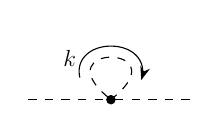
\begin{tikzpicture}[scale=0.7, transform shape, baseline={([yshift=-0.2cm]current bounding box.center)}]
            \begin{feynman}
            \vertex (i) at (-1.5,0);
            \vertex [dot] (v) at (0,0) {};
            \vertex (f) at (1.5,0);
    
            \diagram*{(i) -- [scalar] (v) -- [scalar] (f)};
    
            \draw (v) edge[scalar, loop above, out=140, in=40, min distance=1.5cm, looseness=4, momentum={[arrow distance=4pt]}] (v);
            \node at (-0.75,0.75) {\large $k$};
            \end{feynman}
        \end{tikzpicture}%
}

\newcommand{\BubbleDiagram}[1]{%
\begin{tikzpicture}[scale=0.6, transform shape, baseline={([yshift=-0.1cm]current bounding box.center)}]
\begin{feynman}
    \vertex (i1) at (-1.5,0.8);
    \vertex (i2) at (-1.5,-0.8);
    \vertex [dot] (v1) at (-0.45,0) {};
    \vertex [dot] (v2) at (0.45,0) {};
    \vertex (f1) at (1.5,0.8);
    \vertex (f2) at (1.5,-0.8);

    \diagram*{
        (i1) -- [scalar] (v1),
        (i2) -- [scalar] (v1),
        (v1) -- [scalar, half left, looseness=1.5] (v2),
        (v1) -- [scalar, half right, looseness=1.5] (v2),
        (v2) -- [scalar] (f1),
        (v2) -- [scalar] (f2)
    };
\end{feynman}
\node at (0,-0.8) {$#1$};
\end{tikzpicture}%
}

\newcommand{\DoubleTadpoleDiagram}{
\begin{tikzpicture}[scale=0.7,transform shape,baseline={([yshift=-0.1cm]current bounding box.center)}]
\begin{feynman}
    \vertex (i) at (-1.8,0); 
    \vertex (f) at (1.8,0); 
    \vertex [dot] (v1) at (0,0) {}; 
    \vertex [dot] (v2) at (0,1.2) {}; 
    
    \diagram*{(i)--[scalar](v1)--[scalar](f),(v1)--[scalar,half left,looseness=1.4](v2),(v1)--[scalar,half right,looseness=1.4](v2)}; 
    
    \draw (v2) edge[scalar,loop above,out=140,in=40,min distance=1.3cm,looseness=4] (v2); 

\end{feynman}
\end{tikzpicture}
}

\newcommand{\SunsetDiagram}{
\begin{tikzpicture}[scale=0.7,transform shape,baseline={([yshift=-0.1cm]current bounding box.center)}]
\begin{feynman}
\vertex (i) at (-2,0); 
\vertex [dot] (v1) at (-0.8,0) {}; 
\vertex [dot] (v2) at (0.8,0) {}; 
\vertex (f) at (2,0); 

\diagram*{(i)--[scalar](v1),(v1)--[scalar](v2),(v1)--[scalar,half left,looseness=1.5](v2),(v1)--[scalar,half right,looseness=1.5](v2),(v2)--[scalar](f)}; 

\end{feynman}
\end{tikzpicture}
}

\newcommand{\TadpoleCouplingCT}{
\begin{tikzpicture}[scale=0.7,transform shape,baseline={([yshift=-0.2cm]current bounding box.center)}]
\begin{feynman}
    \vertex (i) at (-1.5,0); 
    \vertex [crossed dot] (v) at (0,0) {}; 
    \vertex (f) at (1.5,0); 
    
    \diagram*{(i)--[scalar](v)--[scalar](f)}; 
    
    \draw (v) edge[scalar,loop above,out=140,in=40,min distance=1.5cm,looseness=4] (v);

\end{feynman}
\end{tikzpicture}
}

\newcommand{\TadpoleMassCT}{
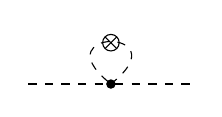
\begin{tikzpicture}[scale=0.7,transform shape,baseline={([yshift=-0.2cm]current bounding box.center)}]
\begin{feynman}
    \vertex (i) at (-1.5,0); 
    \vertex [dot] (v) at (0,0) {}; 
    \vertex (f) at (1.5,0); 
    
    \diagram*{(i)--[scalar](v)--[scalar](f)}; 
    
    \draw (v) edge[scalar,loop above,out=140,in=40,min distance=1.5cm,looseness=4] (v);
    
    \node[crossed dot] at (0,0.75);

\end{feynman}
\end{tikzpicture}
}

\newcommand{\TwoPointCTTwoLoop}{
\begin{tikzpicture}[scale=0.7,transform shape,baseline={([yshift=-0.1cm]current bounding box.center)}]
\begin{feynman}
    \vertex (i) at (-1.5,0); 
    \vertex[crossed dot] (v) at (0,0) {}; 
    \vertex (f) at (1.5,0); 
    
    \diagram*{(i)--[scalar](v)--[scalar](f)};
    
\end{feynman}
\end{tikzpicture}
}

% Double bubble
\newcommand{\FourPointDoubleBubble}{%
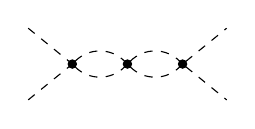
\begin{tikzpicture}[scale=0.7,transform shape,baseline={([yshift=-0.1cm]current bounding box.center)}]
    \begin{feynman}
        \vertex (i1) at (-1.8, 0.65);
        \vertex (i2) at (-1.8,-0.65);

        \vertex[dot] (L) at (-1,0) {};
        \vertex[dot] (C) at ( 0,0) {};
        \vertex[dot] (R) at ( 1,0) {};

        \vertex (f1) at (1.8, 0.65);
        \vertex (f2) at (1.8,-0.65);

        \diagram*{
            (i1) -- [scalar] (L),
            (i2) -- [scalar] (L),

            (L) -- [scalar, bend left=45]  (C),
            (L) -- [scalar, bend right=45] (C),

            (C) -- [scalar, bend left=45]  (R),
            (C) -- [scalar, bend right=45] (R),

            (R) -- [scalar] (f1),
            (R) -- [scalar] (f2)
        };
    \end{feynman}
\end{tikzpicture}%
}

% Overlapping diagram (wineglass)
\newcommand{\FourPointWineglass}{%
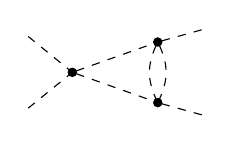
\begin{tikzpicture}[scale=0.7,transform shape,baseline={([yshift=-0.1cm]current bounding box.center)}]
    \begin{feynman}
        \vertex (i1) at (-1.7, 0.65);
        \vertex (i2) at (-1.7,-0.65);

        \vertex[dot] (A) at (-0.9, 0) {};
        \vertex[dot] (B) at ( 0.65, 0.55) {};
        \vertex[dot] (C) at ( 0.65,-0.55) {};

        \vertex (f1) at (1.55, 0.8);
        \vertex (f2) at (1.55,-0.8);

        \diagram*{
            (i1) -- [scalar] (A),
            (i2) -- [scalar] (A),

            (A) -- [scalar] (B),
            (A) -- [scalar] (C),

            (B) -- [scalar, bend left=25]  (C),
            (B) -- [scalar, bend right=25] (C),

            (B) -- [scalar] (f1),
            (C) -- [scalar] (f2)
        };
    \end{feynman}
\end{tikzpicture}%
}

% Bubble with tadpole insertion
\newcommand{\FourPointTadpoleInsertion}{%
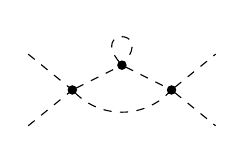
\begin{tikzpicture}[scale=0.7,transform shape,baseline={([yshift=-0.1cm]current bounding box.center)}]
    \begin{feynman}
        \vertex (i1) at (-1.7, 0.65);
        \vertex (i2) at (-1.7,-0.65);

        \vertex[dot] (L) at (-0.9,0) {};
        \vertex[dot] (T) at (0,0.45) {};
        \vertex[dot] (R) at (0.9,0) {};

        \vertex (f1) at (1.7, 0.65);
        \vertex (f2) at (1.7,-0.65);

        \diagram*{
            (i1) -- [scalar] (L),
            (i2) -- [scalar] (L),

            (L) -- [scalar] (T),
            (T) -- [scalar] (R),
            (L) -- [scalar, bend right=45] (R),

            (R) -- [scalar] (f1),
            (R) -- [scalar] (f2)
        };

        \draw (T) edge[scalar, loop above, out=130, in=50, min distance=0.8cm, looseness=4] (T);
        
    \end{feynman}
\end{tikzpicture}%
}

% Bubble with quartic counterterm
\newcommand{\BubbleQuarticCT}{%
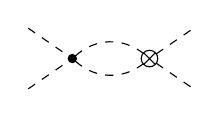
\begin{tikzpicture}[scale=0.7,transform shape,baseline={([yshift=-0.1cm]current bounding box.center)}]
    \begin{feynman}
        \vertex (i1) at (-1.5, 0.55);
        \vertex (i2) at (-1.5,-0.55);

        \vertex[dot] (L) at (-0.7,0) {};
        \vertex[crossed dot]  (R) at ( 0.7,0) {};

        \vertex (f1) at (1.5, 0.55);
        \vertex (f2) at (1.5,-0.55);

        \diagram*{
            (i1) -- [scalar] (L),
            (i2) -- [scalar] (L),

            (L) -- [scalar, bend left=40]  (R),
            (L) -- [scalar, bend right=40] (R),

            (R) -- [scalar] (f1),
            (R) -- [scalar] (f2)
        };
    \end{feynman}
\end{tikzpicture}%
}

% Bubble with mass counterterm insertion
\newcommand{\BubbleMassCT}{%
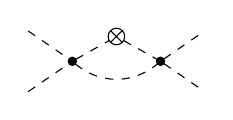
\begin{tikzpicture}[scale=0.7,transform shape,baseline={([yshift=-0.1cm]current bounding box.center)}]
    \begin{feynman}
        \vertex (i1) at (-1.6, 0.55);
        \vertex (i2) at (-1.6,-0.55);

        \vertex[dot] (L) at (-0.8,0) {};
        \vertex[crossed dot]  (M) at (0,0.45) {};
        \vertex[dot] (R) at (0.8,0) {};

        \vertex (f1) at (1.6, 0.55);
        \vertex (f2) at (1.6,-0.55);

        \diagram*{
            (i1) -- [scalar] (L),
            (i2) -- [scalar] (L),

            (L) -- [scalar] (M),
            (M) -- [scalar] (R),
            (L) -- [scalar, bend right=40] (R),

            (R) -- [scalar] (f1),
            (R) -- [scalar] (f2)
        };
    \end{feynman}
\end{tikzpicture}%
}

% tema
\usetheme{Madrid}
\usecolortheme{default}
\usefonttheme{serif}

% numerazione
\setbeamertemplate{headline}{
    \begin{beamercolorbox}[ht=2.5ex,dp=1ex]{section in head/foot}
        \insertsectionnavigationhorizontal{\paperwidth}{}{}
    \end{beamercolorbox}
}
\setbeamertemplate{footline}{
    \leavevmode%
    \hbox{%
        \begin{beamercolorbox}[
            wd=.33\paperwidth,
            ht=2.5ex,
            dp=1ex,
            left
        ]{author in head/foot}
            \hspace{0.3cm}
            \insertshortauthor
        \end{beamercolorbox}%

        \begin{beamercolorbox}[
            wd=.34\paperwidth,
            ht=2.5ex,
            dp=1ex,
            center
        ]{title in head/foot}
            \insertshorttitle
        \end{beamercolorbox}%

        \begin{beamercolorbox}[
            wd=.33\paperwidth,
            ht=2.5ex,
            dp=1ex,
            right
        ]{date in head/foot}
            \insertframenumber/\inserttotalframenumber
            \hspace{0.3cm}
        \end{beamercolorbox}%
    }
}
\setbeamertemplate{navigation symbols}[default]
\setbeamertemplate{blocks}[rounded][shadow=false]

\title{Renormalization of \texorpdfstring{$\phi^4$}{phi4} theory through two loops}
\author{Manuel Gabriele Moretti}
\institute{Physics department \\ Università degli Studi di Torino}
\date{17 september 2026}

\begin{document}

\begin{frame}[plain]
    \titlepage
\end{frame}

\section{Introduction and renormalizability}

\begin{frame}{Bare Lagrangian and Feynman rules}
    \begin{itemize}
        \item A $\phi^4$ theory is a type of self-interaction of a scalar field. The interaction is represented by adding an interaction energy term $-\lambda\phi^4/4!$ to the Lagrangian density. The coupling constant $\lambda$ is dimensionless in 4-dimensional spacetime. The bare Lagrangian of a scalar $\phi^4$ theory is
        \begin{equation}
        \label{eq: bare Lagrangian}
        \Lag_0 = \frac{1}{2}\p_\mu\phi_0\p^\mu\phi_0 - \frac{1}{2}m_0^2\phi_0^2 - \frac{\lambda_0}{4!}\phi^4.
        \end{equation}
    By looking at the bare Lagrangian \eqref{eq: bare Lagrangian}, we can see that the theory has a global $\mathbb{Z}_2$ symmetry mapping $\phi \to -\phi$, which forbids interaction terms containing an odd number of scalar fields.
    \item We can now compute the Feynman rules, these are\supcite{Collins}:
    \begin{enumerate}
        \item for each internal scalar line with momentum $p$ we have
        \begin{equation}
            \ScalarPropagator = \frac{i}{p^2 - m_0^2 + i\varnothing^+};
        \end{equation}
        \item for each four-scalar interaction vertex we have
        \begin{equation}
            \FourScalarVertex = -i\lambda_0.
        \end{equation}
    \end{enumerate}
    \end{itemize}
\end{frame}

\begin{frame}{Superficial degree of divergence and divergent diagrams at one loop}
    \begin{itemize}
        \item For a generic scalar field theory with a Lagrangian of interaction $\Lag_i = -\lambda \phi^p/p!$, the superficial degree of divergence can be expressed as $\omega(\Gamma) = D - E([\phi]/[m]) - V([\lambda]/[m])$, where
    \begin{equation}
        \frac{[\phi]}{[m]} = \frac{D - 2}{2},\quad \frac{[\lambda]}{[m]} = D - p\frac{D - 2}{2}.
    \end{equation}
    In the case of $\phi^4$ theory, we have $p = 4$ and $D = 4$, thus $[\phi]/[m] = 1$ and $[\lambda]/[m] = 0$, so the theory is renormalizable. 
    \item For a diagram with $E$ external lines and $V$ vertices, $\omega(\Gamma)$ in $D = 4$ is then given by $\omega(\Gamma) = 4 - E$. We can now identify the potentially UV-divergent diagrams at 1-loop.
    \begin{table}[]
        \centering
        \begin{tabular}{|c|c|c|c|c|}
            \hline
             & $E$ & $\omega(\Gamma)$ & $S$ & name \\
             \hline
             \TadpoleDiagram & 2 & 2 & 2 & tadpole \\
             \BubbleDiagram{} & 4 & 0 & 2 & bubble \\
             \hline
        \end{tabular}
        \label{tab: divergent diagrams}
    \end{table}
    \end{itemize}
\end{frame}

\section{Renormalization at one loop}

\begin{frame}{Bubble contribution and renormalized quantities}
    \begin{itemize}
        \item The tadpole contribution to the 2-point function is quadratically UV-divergent while the bubble contribution to the 4-point function is logarithmically UV-divergent. For the latter, since the external momenta can be distributed in three inequivalent ways, there are three diagrams: the $s$-channel, the $t$-channel, and the $u$-channel; thus
        \begin{equation}
        \label{eq: bubble contribution}
            \BubbleDiagram{} = \BubbleDiagram{s} + \BubbleDiagram{t} + \BubbleDiagram{u}
        \end{equation}
        Also, all 1-loop diagrams with $E \ge 6$ are superficially UV-finite.
        \item  After introducing dimensional regularization, the dimensions of the bare field, mass and coupling are $[\phi_0] = 1 - \epsilon$, $ [m_0] = 1$, and $[\lambda_0] = 2\epsilon$. We now introduce renormalized quantities\supcite{Peskin} through
        \begin{equation}
            \phi_0 = Z_\phi^{1/2}\phi_R,\quad m_0^2 = Z_m m_R^2,\quad \lambda_0 = \mu_R^{2\epsilon}Z_\lambda\lambda_R.
        \end{equation}
        The scale $\mu_R$ has mass dimension one and ensures that the renormalized coupling $\lambda_R$ remains dimensionless.
    \end{itemize}
\end{frame}

\begin{frame}{Renormalized and counter-term Lagrangians}
    Substituting the renormalized quantities into the bare Lagrangian \eqref{eq: bare Lagrangian} we obtain
    \begin{equation}
        \Lag_0 = \frac{1}{2}Z_\phi(\p_\mu\phi_R)(\p^\mu\phi_R) - \frac{1}{2}Z_\phi Z_m m_R^2\phi_R^2 -\frac{\mu_R^{2\epsilon}\lambda_R}{4!}Z_\lambda Z_\phi^2\phi_R^4.
    \end{equation}
    The bare Lagrangian can then be decomposed as $\Lag_0 = \Lag_R + \Lag_{CT}$, where the renormalized and the counter-term Lagrangians are  
    \begin{equation}
        \Lag_R = \frac{1}{2}(\p_\mu\phi_R)^2 - \frac{1}{2}m_R^2\phi_R^2 - \frac{\mu_R^{2\epsilon}\lambda_R}{4!}\phi_R^4,
    \end{equation}
    \begin{equation}
        \Lag_{CT} = \frac{1}{2}\delta_1(\p_\mu\phi_R)^2 - \frac{1}{2}\delta_2m_R^2\phi_R^2 - \delta_3\frac{\lambda_R\mu_R^{2\epsilon}}{4!}\phi_R^4
    \end{equation}
    where we have set $Z_1 \equiv Z_\phi$, $Z_2 \equiv Z_\phi Z_m$, $Z_3 \equiv Z_\lambda Z_\phi^2$ and defined the counter-terms as
    \begin{equation}
        \delta_x = Z_x - 1,\quad x = \{1,2,3\}.
    \end{equation}
\end{frame}

\begin{frame}{Counter-term Feynman rules}
    The counter-term Lagrangian introduces additional interaction vertices, these are:
    \begin{itemize}
        \item The 2-point counter-term vertex
        \begin{equation}
            \ScalarPropagatorCounterterm{} = i(\delta_1p^2-\delta_2m_R^2),
        \end{equation}
        where term proportional to $\delta_1$ renormalizes the kinetic term, while the one proportional to $\delta_2$ renormalizes the mass;
        \item the 4-point counter-term vertex
        \begin{equation}
            \FourScalarVertexCounterterm{} = -i\mu_R^{2\epsilon}\lambda_R\delta_3.
        \end{equation}
    \end{itemize}
    The counter-terms admit a loop expansion $\delta_x = \delta_x^{(1)} + \delta_x^{(2)} + \cdots$, so at every order they can be fixed by requiring the renormalized correlation functions to be UV finite.
\end{frame}

\begin{frame}{2- and 4-point function contributions at one loop}
    The 1-loop contribution to the 2-point function from the tadpole diagram is\supcite[Eq.~(8.62)]{Kleinert}
    \begin{equation}
        \begin{aligned}
        \label{eq: tadpole contribution}
            \TadpoleDiagramMomentum &= \frac{1}{2}(-i\mu_R^{2\epsilon}\lambda_R) \int_k\frac{i}{k^2-m_R^2+i0^+} \\
            &= \frac{i\lambda_Rm_R^2}{32\pi^2}\bigg[\frac{1}{\epsilon} - \gamma_E + \log(4\pi) + 1 - \log\bigg(\frac{m_R^2}{\mu_R^2}\bigg)\bigg] + O(\epsilon).
        \end{aligned}
    \end{equation}
    The 4-point function receives three bubble contributions, corresponding to the $s$-, $t$- and $u$-channels. For a generic channel with momentum $q$, the contribution is\supcite[Eq.~(8.68)]{Kleinert}
    \begin{equation}
    \label{eq: general bubble contribution}
        \begin{aligned}
            \BubbleDiagram{q} &= \frac{1}{2}(-i\mu_R^{2\epsilon}\lambda_R)^2\int_k\frac{i}{k^2-m_R^2+i0^+}\frac{i}{(k+q)^2-m_R^2+i0^+} \\
            &= \frac{i\lambda_R^2\mu_R^{2\epsilon}}{32\pi^2}\bigg[\frac{1}{\epsilon} - \gamma_E + \log(4\pi) + \log{\bigg(\frac{\mu_R^2}{m_R^2}\bigg)} + 2 - \beta_q\log{\bigg(\frac{\beta_{q,+}}{\beta_{q,-}}\bigg)} \bigg] + O(\epsilon).
        \end{aligned}
    \end{equation}
    To get the whole contribution we then need to sum over the three channels the expression \eqref{eq: general bubble contribution}, namely over $q^2 \in \{s,t,u\}$.
\end{frame}

\begin{frame}{2-point function counter-terms}
    From the result in \eqref{eq: tadpole contribution}, the 1-loop tadpole contribution UV-divergent part is
    \begin{equation}
        T^{(1)}_{\mathrm{UV}} \equiv \frac{i\lambda_Rm_R^2}{32\pi^2}\frac{1}{\bepsilon},\quad \frac{1}{\bepsilon} \equiv \frac{1}{\epsilon} - \gamma_E + \log(4\pi).
    \end{equation}
    Since the tadpole is independent of the external momentum $p$, it produces no UV divergence proportional to $p^2$. Therefore,
    \begin{equation}
        \delta_1^{(1)} = 0.
    \end{equation}
    The remaining divergence is proportional to $m_R^2$ and must be cancelled by the mass counter-term. Requiring UV finiteness, using $\Gamma_{2,\mathrm{CT}}^{(1)} \equiv \ScalarPropagatorCounterterm{(1)} = -i\delta_2^{(1)}m_R^2,$ means requiring cancellation of the UV divergence through
    \begin{equation}
        T^{(1)}_{\mathrm{UV}} + \Gamma_{2,\mathrm{CT}}^{(1)} = \frac{i\lambda_Rm_R^2}{32\pi^2}\frac{1}{\bepsilon} - i\delta_2^{(1)}m_R^2 = 0.
    \end{equation}
    Therefore, in the $\MMS$ scheme,
    \begin{equation}
        \delta_2^{(1)} = \frac{\lambda_R}{32\pi^2}\frac{1}{\bepsilon}.
    \end{equation}
\end{frame}

\begin{frame}{4-point function counter-term}
    From the result in \eqref{eq: general bubble contribution}, the pole is independent of the channel momentum, so each diagram has the same UV-divergent part
    \begin{equation}
        B_{q,\mathrm{UV}}^{(1)} = \frac{i\lambda_R^2\mu_R^{2\epsilon}}{32\pi^2}\frac{1}{\bar{\epsilon}},
    \end{equation}
    so summing the three channels gives a total contribution of $\sum\nolimits_qB_{4,q}^{(1)} \equiv B_{4}^{(1)} = 3B^{(1)}_{4,q}$. The sum of the three bubble divergences is cancelled by the 4-point counter-term
    \begin{equation}
        \Gamma_{4,\mathrm{CT}}^{(1)} \equiv \FourScalarVertexCounterterm{(1)} = -i\lambda_R\mu_R^{2\epsilon}\delta_3^{(1)},
    \end{equation}
    Requiring cancellation of the UV divergence through
    \begin{equation}
        B_{4}^{(1)} + \Gamma_{4,\mathrm{CT}}^{(1)} = \frac{3i\lambda_R^2\mu_R^{2\epsilon}}{32\pi^2}\frac{1}{\bar{\epsilon}} - i\lambda_R\mu_R^{2\epsilon}\delta_3^{(1)} = 0,
    \end{equation}
    gives, in the $\MMS$ scheme,
    \begin{equation}
        \delta_3^{(1)} = \frac{3\lambda_R}{32\pi^2}\frac{1}{\bar{\epsilon}}.
    \end{equation}
\end{frame}

\begin{frame}{Renormalization constants at one loop}
    From the renormalization of the 2- and 4-point functions at 1-loop, we have obtained
    \begin{equation}
    \label{eq: counter-terms at 1-loop}
        \delta_1^{(1)}=0,\quad \delta_2^{(1)}=\frac{\lambda_R}{32\pi^2}\frac{1}{\bar{\epsilon}},\quad \delta_3^{(1)}=\frac{3\lambda_R}{32\pi^2}\frac{1}{\bar{\epsilon}}.
    \end{equation}
    Since $Z_x = 1 + \delta_x$, the corresponding renormalization constants are
    \begin{equation}
        Z_1 = 1 + O(\lambda_R^2),\quad Z_2 = 1 + \frac{\lambda_R}{32\pi^2}\frac{1}{\bar{\epsilon}} + O(\lambda_R^2),\quad Z_3 = 1 + \frac{3\lambda_R}{32\pi^2}\frac{1}{\bar{\epsilon}}+O(\lambda_R^2).
    \end{equation}
    Recalling that $Z_\phi = Z_1$, $Z_\phi Z_m = Z_2$, and $Z_\lambda Z_\phi^2 = Z_3$, we finally obtain
    \begin{equation}
    \label{eq: renormalization constants Zphi, Zm, and Zlambda}
        Z_\phi = 1 + O(\lambda_R^2),\quad Z_m = 1 + \frac{\lambda_R}{32\pi^2}\frac{1}{\bar{\epsilon}}+ O(\lambda_R^2),\quad Z_\lambda = 1 + \frac{3\lambda_R}{32\pi^2}\frac{1}{\bar{\epsilon}} + O(\lambda_R^2).
    \end{equation}
    These constants cancel all the 1-loop UV divergences of the $\phi^4$ theory.
\end{frame}

\begin{frame}{Running coupling at one loop}
\setlength{\belowdisplayskip}{2pt}
    The bare coupling $\lambda_0 = \mu_R^{2\epsilon}Z_\lambda\lambda_R$ cannot depend on the arbitrary renormalization scale $\mu_R$. Therefore, knowing the beta function $\beta(\lambda_R)$ definition and using the fact that, in the $\MMS$ scheme, $Z_\lambda$ found in \eqref{eq: renormalization constants Zphi, Zm, and Zlambda} depends on $\mu_R$ only through $\lambda_R$, we obtain that
    \begin{equation}
        \mu_R\frac{d\lambda_0}{d\mu_R} = 2\epsilon\lambda_R Z_\lambda+\beta(\lambda_R)\left(Z_\lambda+\lambda_R\frac{\partial Z_\lambda}{\partial\lambda_R}\right) = 0 \quad \Rightarrow \quad \beta(\lambda_R) = \frac{3\lambda_R^2}{16\pi^2} + O(\lambda_R^3),
    \end{equation}
    in the physical limit $D \to 4$, or equivalently for $\epsilon \to 0$. The positive sign shows that the $\phi^4$ coupling increases with the renormalization scale. Thus, the renormalization group equation for the $\phi^4$ theory is
    \begin{equation}
        \mu_R\frac{d\lambda_R}{d\mu_R} = \frac{3\lambda_R^2}{16\pi^2}.
    \end{equation}
    From separating the variables, integrating between a reference scale $\mu_0$ and a generic scale $\mu_R$, and solving for $\lambda_R(\mu_R)$, we obtain that the running coupling is 
    \begin{equation}
        \lambda_R(\mu_R)=\frac{\lambda_R(\mu_0)}{1-\dfrac{3\lambda_R(\mu_0)}{16\pi^2}\log\left(\dfrac{\mu_R}{\mu_0}\right)}.
    \end{equation}
\end{frame}

\section{Renormalization at two loops}

\begin{frame}{Divergent 2-point diagrams at two loops}
For a connected 2-point diagram at 2-loop, the numbers of internal lines and vertices are given by $4V = 2I + E$, thus $I = 3$ and $V = 2$. There are two potentially divergent diagrams\supcite[Eq.~(8.53)]{Kleinert}.
\begin{table}[]
    \centering
    \begin{tabular}{|c|c|c|c|c|}
        \hline
         & $E$ & $\omega(\Gamma)$ & $S$ & name \\ \hline
         \DoubleTadpoleDiagram & 2 & 2 & 4 & double tadpole \\ 
         \SunsetDiagram & 2 & 2 & 6 & sunset \\ 
         \hline
    \end{tabular}
    \label{tab: 2-loop divergent graphs}
\end{table}
\begin{itemize}
    \item Regarding the double tadpole, no external momentum flows through the loops: its contribution is independent of $p$ and can only renormalize the mass.
    \item Regarding the sunset, the external momentum flows through the internal lines: its divergent part can contain both $m_R^2$ and $p^2$ terms.
\end{itemize}
% commento utile
% A connected graph in which two tadpoles are joined by a single propagator is one-particle reducible and is not part of the 1PI self-energy.
\end{frame}

\begin{frame}{Divergent 4-point diagrams at two loops}
    For a connected 4-point diagram at 2-loop, the number of internal lines and vertices are given by $4V = 2I + E$, thus $I=4$ and $V=3$. There are three potentially divergent diagrams\supcite[Eq.~(8.54)]{Kleinert}.
    \begin{table}
        \centering
        \begin{tabular}{|c|c|c|c|c|}
            \hline
            diagram & $E$ & $\omega(\Gamma)$ & $S$ & name \\
            \hline
            \FourPointDoubleBubble & $4$ & $0$ & $4$ & double bubble \\
            \FourPointWineglass & $4$ & $0$ & $2$ & wineglass \\
            \FourPointTadpoleInsertion & $4$ & $0$ & $2$ & tadpole insertion \\
            \hline
        \end{tabular}
    \end{table}
    \begin{itemize}
        \item The double bubble and wineglass diagrams contain 1-loop bubble sub-graphs.
        \item The tadpole insertion diagram contains a 1-loop tadpole sub-graph.
    \end{itemize}
\end{frame}

\begin{frame}{Sub-divergences at two loops}
    % commento utile
    % A sub-divergence is a UV divergence associated with a proper 1PI sub-diagram $\gamma\subset\Gamma$.
    For the 2-point function:
    \begin{itemize}
        \item The double tadpole contains a divergent 1-loop tadpole sub-diagram and a divergent 1-loop bubble sub-diagram.
        \item The sunset contains three overlapping logarithmically divergent 1-loop bubble sub-diagrams, obtained by selecting any two of its three internal propagators.
    \end{itemize}
    For the 4-point function:
    \begin{itemize}
        \item The double bubble contains two divergent 1-loop bubble sub-diagrams.
        \item The wineglass contains one divergent 1-loop bubble sub-diagram.
        \item The tadpole-insertion diagram contains a divergent 1-loop tadpole sub-diagram.
    \end{itemize}
    All the 1-loop sub-divergences must be removed before treating the 2-loop divergences. In particular, the 1-loop mass counter-term $\delta_2^{(1)}$ cancels tadpole sub-divergences, while the 1-loop vertex counter-term $\delta_3^{(1)}$ cancels bubble sub-divergences. Thus, only the remaining local pole is assigned to a 2-loop counter-term.
\end{frame}

\begin{frame}{Counter-term Feynman rules at \texorpdfstring{$n$}{n} loops}
    Using the loop expansion for $\delta_x$, the vertex structure does not change with the loop order. At loop order $n$, the counter-term Feynman rules are:
    \begin{itemize}
        \item the 2-point counter-term vertex is
        \begin{equation}
            \Gamma^{(n)}_{2,\mathrm{CT}} = \ScalarPropagatorCounterterm{(n)} = i(\delta_1^{(n)}p^2-\delta_2^{(n)}m_R^2);
        \end{equation}
        \item the 4-point counter-term vertex is
        \begin{equation}
            \Gamma^{(n)}_{4,\mathrm{CT}} \equiv \FourScalarVertexCounterterm{(n)} = -i\mu_R^{2\epsilon}\lambda_R\delta_3^{(n)}.
        \end{equation}
    \end{itemize}
    Therefore, in general at 2-loop order, vertices proportional to $\delta_x^{(1)}$ are inserted into 2-loop diagrams to cancel their sub-divergences, while vertices proportional to $\delta_x^{(2)}$ cancel the remaining overall divergences\supcite{Collins}.
\end{frame}

\begin{frame}{2-point function counter-term insertions}
    Using the results \eqref{eq: counter-terms at 1-loop} in the $\MMS$ scheme, recalling the 1-loop tadpole contribution \eqref{eq: tadpole contribution}, and setting $F_T \equiv 1 - \log(m_R^2/\mu_R^2)$, we have
    \begin{equation}
        \Sigma_{\delta_3^{(1)}}^{(2)} \equiv \TadpoleCouplingCT = -\frac{i\mu_R^{2\epsilon}\lambda_R\delta_3^{(1)}}{2}\int_k\frac{i}{D_k} = \frac{3i\lambda_R^2m_R^2}{(32\pi^2)^2}\left[\frac{1}{\bepsilon^2} + \frac{F_T}{\bepsilon}\right] + O(\epsilon^0),
    \end{equation}
    \begin{equation}
        \Sigma_{\delta_2^{(1)}}^{(2)} \equiv \TadpoleMassCT = -\frac{i\mu_R^{2\epsilon}\lambda_R}{2}\int_k\frac{i}{D_k}(-i\delta_2^{(1)}m_R^2)\frac{i}{D_k} = \frac{i\lambda_R^2m_R^2}{(32\pi^2)^2}\left[\frac{1}{\bepsilon^2} + \frac{F_T - 1}{\bepsilon}\right] + O(\epsilon^0).
    \end{equation}
    The complete contribution at order $\lambda_R^2$ is
    \begin{equation}
        \begin{aligned}
            \Sigma_R^{(2)} &= \Sigma_{\mathrm{DT}}^{(2)} + \Sigma_{\mathrm{sun}}^{(2)} + \Sigma_{\delta_3^{(1)}}^{(2)} + \Sigma_{\delta_2^{(1)}}^{(2)} + i(\delta_1^{(2)}p^2-\delta_2^{(2)}m_R^2) \\
            &\equiv \Sigma_{\mathrm{sub}}^{(2)}(p^2) + i(\delta_1^{(2)}p^2-\delta_2^{(2)}m_R^2).
        \end{aligned}
    \end{equation}
\end{frame}

\begin{frame}{4-point function counter-term insertions}
    Recalling the 1-loop bubble contribution \eqref{eq: general bubble contribution}, we have
    \begin{equation}
        \begin{aligned}
            \Gamma_{4,\delta_3^{(1)}}^{(2)}(q) = \BubbleQuarticCT &= (-i\mu_R^{2\epsilon}\lambda_R)(-i\mu_R^{2\epsilon}\lambda_R\delta_3^{(1)})\int_k\frac{i}{D_k}\frac{i}{D_{k+q}} \\
            &= \frac{6i\mu_R^{2\epsilon}\lambda_R^3}{(32\pi^2)^2}\left[\frac{1}{\bepsilon^2} + F_B(q^2)\frac{1}{\bepsilon}\right] + O(\epsilon^0),
        \end{aligned}
    \end{equation}
    \begin{equation}
        \begin{aligned}
            \Gamma_{4,\delta_2^{(1)}}^{(2)}(q) = \BubbleMassCT &= (-i\mu_R^{2\epsilon}\lambda_R)^2\int_k\frac{i}{D_k}(-i\delta_2^{(1)}m_R^2)\frac{i}{D_k}\frac{i}{D_{k+q}} \\
            &= \frac{i\mu_R^{2\epsilon}\lambda_R^3}{(32\pi^2)^2}\frac{1}{\bepsilon}\,m_R^2\frac{\partial F_B(q^2)}{\partial m_R^2} + O(\epsilon^0),
        \end{aligned}
    \end{equation}
    where $F_B(q^2)$ is the finite part obtained in the 1-loop result \eqref{eq: general bubble contribution}. The complete contribution at order $\lambda_R^3$ is
    \begin{equation}
        \Gamma_{4,R}^{(2)} = \Gamma_{\mathrm{DB}}^{(2)} + \Gamma_{\mathrm{WG}}^{(2)} + \Gamma_{\mathrm{TI}}^{(2)} + \Gamma_{4,\delta_3^{(1)}}^{(2)} + \Gamma_{4,\delta_2^{(1)}}^{(2)} - i\mu_R^{2\epsilon}\lambda_R\delta_3^{(2)} \equiv \Gamma_{4,\mathrm{sub}}^{(2)} - i\mu_R^{2\epsilon}\lambda_R\delta_3^{(2)}.
    \end{equation}
\end{frame}

\begin{frame}{Double tadpole and sunset contributions}
    \begin{itemize}
        \item Assigning momentum $k$ to the two propagators connecting the vertices and momentum $\ell$ to the upper tadpole, the double tadpole contribution is given by\supcite[Eq.~(8.72)]{Kleinert}
        \begin{equation}
            \begin{aligned}
                \Sigma^{(2)}_{\mathrm{DT}}  &= \frac{(-i\lambda_R\mu_R^{2\epsilon})^2}{4} \int_k\int_\ell\frac{i^3}{D(k,m_R)^2D(\ell,m_R)} \\
                &= -\frac{i\lambda_R^2m_R^2}{4(16\pi^2)^2}\bigg[\frac{1}{\bar{\epsilon}^2} + \frac{1-2\log{(m_R^2/\mu_R^2)}}{\bar{\epsilon}}\bigg] + O(\epsilon^0);
            \end{aligned}
        \end{equation}
        \item Assigning momentum $k$, $\ell$ and $p - k -\ell$ to the three internal lines, the sunset contribution is hard to compute since the integrals do not factorise, so we report just the result\supcite[Eq.~(8.96)]{Kleinert}
        \begin{equation}
            \Sigma^{(2)}_{\mathrm{sun}} \equiv \frac{i\lambda_R^2}{(16\pi^2)^2}\bigg\{m_R^2\bigg[-\frac{1}{4\bepsilon^2} + \bigg(-\frac{3}{4} + \frac{1}{2}\log{\frac{m_R^2}{\mu_R^2}}\bigg)\frac{1}{\bepsilon}\bigg] + \frac{p^2}{24\bepsilon}\bigg\} + O(\epsilon^0).
        \end{equation}
    \end{itemize}
    The double pole of the double tadpole originates from nested 1-loop UV divergences. The sunset instead contains overlapping 1-loop 4-point sub-divergences, cancelled by the counter-term $\delta_3^{(1)}$.
\end{frame}

\begin{frame}{2-loop mass and field counter-terms}
After the cancellation of all sub-divergences, the remaining UV-divergent part of $\Sigma_{\mathrm{sub}}^{(2)}$ is
\begin{equation}
    \Sigma_{\mathrm{sub,UV}}^{(2)}(p^2) = \frac{i\lambda_R^2}{(16\pi^2)^2}\bigg[m_R^2\bigg(\frac{1}{2\bepsilon^2}-\frac{1}{4\bepsilon}\bigg)+\frac{p^2}{24\bepsilon}\bigg].
\end{equation}
Requiring the cancellation of said UV divergence through
\begin{equation}
    \Sigma_{\mathrm{sub,UV}}^{(2)}(p^2) + \Gamma_{2,\mathrm{CT}}^{(2)} = 0,
\end{equation}
matching separately the coefficients of $m_R^2$ and $p^2$, gives
\begin{equation}
\label{eq: counter-term 1 and 2 at 2-loop}
    \delta_1^{(2)} = -\frac{\lambda_R^2}{24(16\pi^2)^2}\frac{1}{\bepsilon},\quad \delta_2^{(2)} = \frac{\lambda_R^2}{(16\pi^2)^2}\bigg[\frac{1}{2\bepsilon^2} - \frac{1}{4\bepsilon}\bigg].
\end{equation}
The mass divergence receives contributions from all the diagrams, whereas the $p^2$ pole originates only from the sunset. Therefore, field renormalization vanishes at one loop but becomes non-zero at two loops.
\end{frame}

\begin{frame}{2-loop coupling counter-term}
\setlength{\belowdisplayskip}{2pt}
% commento utile
% After adding the 1-loop counter-term insertions, all non-local poles associated with the sub-divergences cancel. Since the superficial degree of divergence is $\omega = 0$, the remaining overall divergence is independent of the external momenta and has the same local structure as the operator $\phi_R^4$.
The explicit evaluation of the 2-loop 4-point integrals is onerous. 
% commento utile
% Since we are interested in UV renormalization, we quote only their combined pole part after the subtraction of the 1-loop sub-divergences.
So, after the cancellation of all sub-divergences and including all inequivalent assignments of the external momenta\supcite[Sec.~8.3.3]{Kleinert}, we report just the UV-divergent part of $\Gamma_{4,\mathrm{sub}}^{(2)}$ which is
\begin{equation}
    \Gamma_{4,\mathrm{sub,UV}}^{(2)} = \frac{i\mu_R^{2\epsilon}\lambda_R^3}{(16\pi^2)^2}\bigg[\frac{9}{4\bepsilon^2} - \frac{3}{2\bepsilon}\bigg].
\end{equation}
The double pole is fixed by the nested 1-loop sub-divergences, whereas the simple pole represents the new 2-loop divergence. Requiring cancellation of the remaining UV divergence through
\begin{equation}
    \Gamma_{4,\mathrm{sub,UV}}^{(2)} - i\mu_R^{2\epsilon}\lambda_R\delta_3^{(2)} = 0,
\end{equation}
gives
\begin{equation}
    \delta_3^{(2)} = \frac{\lambda_R^2}{(16\pi^2)^2}\bigg[\frac{9}{4\bepsilon^2} - \frac{3}{2\bepsilon}\bigg].
\end{equation}
Recalling that $Z_\lambda = Z_3/Z_\phi^2$ and using the results at 2-loop \eqref{eq: counter-term 1 and 2 at 2-loop}, we get 
\begin{equation}
    Z_\lambda = 1 + \frac{3\lambda_R}{32\pi^2}\frac1{\bepsilon} + \frac{\lambda_R^2}{(16\pi^2)^2}\bigg[\frac{9}{4\bepsilon^2} - \frac{17}{12\bepsilon}\bigg] + O(\lambda_R^3).
\end{equation}
\end{frame}

\section{Conclusions}

\begin{frame}{Renormalization constants through two loops}
\begin{itemize}
    \item In $D = 4 - 2\epsilon$, the only superficially divergent 1PI functions with external legs are the 2-point and 4-point functions.
    \item At one loop, the tadpole renormalizes the mass, while the $s$-, $t$- and $u$-channel bubbles renormalize the quartic vertex. Since the tadpole is independent of the external momentum, field renormalization starts only at two loops.
    \item In the $\MMS$ scheme, the renormalization constants up to 2-loop order are
    \begin{equation}
        Z_1 = 1 - \frac{\lambda_R^2}{24(16\pi^2)^2}\frac{1}{\bar{\epsilon}} + O(\lambda_R^3),\quad Z_2 = 1 + \frac{\lambda_R}{32\pi^2}\frac{1}{\bar{\epsilon}} + \frac{\lambda_R^2}{(16\pi^2)^2}\bigg[\frac{1}{2\bar{\epsilon}^2} - \frac{1}{4\bar{\epsilon}}\bigg] + O(\lambda_R^3)
    \end{equation}
    \begin{equation}
        Z_3 = 1+\frac{3\lambda_R}{32\pi^2}\frac{1}{\bar{\epsilon}} + \frac{\lambda_R^2}{(16\pi^2)^2}\bigg[\frac{9}{4\bar{\epsilon}^2} - \frac{3}{2\bar{\epsilon}}\bigg] + O(\lambda_R^3).
    \end{equation}
\end{itemize}
These renormalization constants cancel all remaining UV poles of the 2-point and 4-point functions through two-loop order.
\end{frame}

\begin{frame}{Structure of 2-loop renormalization}
The 2-loop calculation illustrates the general structure of perturbative renormalization\supcite{Collins}:
\begin{itemize}
    \item 1-loop counter-term insertions cancel the sub-divergences of the 2-loop diagrams;
    \item the remaining overall divergences are local and are removed by the operators already present in the Lagrangian;
    \item double poles originate from nested 1-loop sub-divergences, whereas simple poles contain genuinely new 2-loop information;
\end{itemize}
Using the 2-loop results for $Z_\lambda$ and $Z_\phi$, together with the same scale-independence argument employed at 1-loop, the renormalization-group functions up to this order are\supcite[Eqs.~(8)--(9)]{KleinertRG}
\begin{equation}
\label{eq: 2-loop beta and gamma function}
    \beta(\lambda_R) = \frac{3\lambda_R^2}{16\pi^2} - \frac{17\lambda_R^3}{3(16\pi^2)^2} + O(\lambda_R^4), \quad \gamma_\phi(\lambda_R) = \frac{\lambda_R^2}{12(16\pi^2)^2} + O(\lambda_R^3).
\end{equation}
Since the leading coefficient of $\beta(\lambda_R)$ is positive, the coupling increases towards high energies and the theory is not asymptotically free.
\end{frame}

\begin{frame}{Running coupling through two loops}
    \begin{columns}[T,onlytextwidth]
    \begin{column}{0.45\textwidth}
    The 2-loop beta function is in \eqref{eq: 2-loop beta and gamma function}. Setting
    \begin{equation}
        L \equiv \log\frac{\mu_R}{\mu_0},\quad w \equiv 1 - \frac{3\lambda_R(\mu_0)L}{16\pi^2},
    \end{equation}
    the 1- and 2-loop solutions are
    \begin{equation}
        \lambda_R^{(1)} = \frac{\lambda_R(\mu_0)}{w},
    \end{equation}
    \begin{equation}
        \lambda_R^{(2)} = \frac{\lambda_R(\mu_0)}{w} + \frac{17\lambda_R^2(\mu_0)}{144\pi^2}\frac{\log w}{w^2}
    \end{equation}
    The negative 2-loop correction slows the growth of the coupling. The result is reliable only in the perturbative region, so for
    $\lambda_R/(16\pi^2) \ll 1$. The theory remains not asymptotically free.
    \end{column}

    \begin{column}{0.53\textwidth}
    \centering
        \begin{tikzpicture}
        \begin{axis}[width=\linewidth, height=0.60\textheight, xlabel={$\mu_R/\mu_0$}, ylabel={$\lambda_R(\mu_R)$}, xmode=log, xmin=1, xmax=1000, ymin=4.5, ymax=15, grid=major, title={illustrative choice: $\lambda_R(\mu_0) = 5$}, title style={font=\small}, legend style={font=\scriptsize, draw=none, fill=none, at={(0.03,0.97)}, anchor=north west}]
        
        \def\lamref{5}
        
        \addplot[blue, very thick, domain=1:1000, samples=200]{\lamref/(1-3*\lamref*ln(x)/(16*pi^2))};
        
        \addlegendentry{$\lambda_R^{(1)}$}
        
        \addplot[red, very thick, dashed, domain=1:1000,samples=200]
        {\lamref/(1-3*\lamref*ln(x)/(16*pi^2)) + (17*\lamref^2)/(144*pi^2)*ln(1-3*\lamref*ln(x)/(16*pi^2))/(1 - 3*\lamref*ln(x)/(16*pi^2))^2};
        
        \addlegendentry{$\lambda_R^{(2)}$}
        
        \end{axis}
        \end{tikzpicture}
    \end{column}
    \end{columns}
\end{frame}

\begin{frame}{Bibliography}
\footnotesize
\setbeamertemplate{bibliography item}[text]

\begin{thebibliography}{9}

\bibitem{Peskin}
M.~E.~Peskin and D.~V.~Schroeder,
\emph{An Introduction to Quantum Field Theory},
Addison-Wesley, 1995.

\bibitem{Kleinert}
H.~Kleinert and V.~Schulte-Frohlinde,
\emph{Critical Properties of $\phi^4$-Theories},
World Scientific, 2001.

\bibitem{Collins}
J.~C.~Collins,
\emph{Renormalization: general theory},
2006.
\href{https://arxiv.org/abs/hep-th/0602121}{arXiv:hep-th/0602121}.

\bibitem{KleinertRG}
H.~Kleinert, J.~Neu, V.~Schulte-Frohlinde, K.~G.~Chetyrkin and S.~A.~Larin,
\emph{Five-loop renormalization group functions of $O(n)$-symmetric $\phi^4$-theory and $\epsilon$-expansions of critical exponents up to $\epsilon^5$},
Phys.\ Lett.\ B \textbf{272}, 39--44 (1991);
Erratum: Phys.\ Lett.\ B \textbf{319}, 545 (1993).
\href{https://arxiv.org/abs/hep-th/9503230}{arXiv:hep-th/9503230}.

\end{thebibliography}
\end{frame}

% APPENDIX

\appendix
\section{Appendix}

\setcounter{equation}{0}
\renewcommand{\theequation}{A.\arabic{equation}}

\newcommand{\Kloop}{(16\pi^2)}
\newcommand{\Lmass}{L_m}
\newcommand{\appref}[1]{\par\smallskip{\scriptsize #1}}


\begin{frame}{Evaluation of the loop integrals}

The aim of this appendix is to show the main steps used to evaluate
the loop integrals entering the one- and two-loop renormalization
of $\phi^4$ theory.

\begin{equation}
D=4-2\epsilon,
\qquad
\int_k \equiv \int\frac{d^Dk}{(2\pi)^D},
\qquad
D_k=k^2-m_R^2+i0^+ .
\end{equation}

We also define
\begin{equation}
c=\log(4\pi)-\gamma_E,
\qquad
\frac1{\bar\epsilon}
=
\frac1\epsilon+c,
\qquad
\Lmass=\log\frac{m_R^2}{\mu_R^2}.
\end{equation}

At two loops only the UV divergent terms are retained:
\begin{equation}
\frac1{\epsilon^2},
\qquad
\frac1{\epsilon}.
\end{equation}

Finite two-loop remainders are not required for the determination
of the counter-terms.

\appref{The calculation follows the methods of Ref.~\cite{Kleinert},
in particular the evaluation of loop integrals through Feynman
parameters and endpoint singularities.}

\end{frame}


\begin{frame}{Dimensionally regularized 1-loop master integral}

After a Wick rotation, consider the Euclidean integral
\begin{equation}
J_a^{[D]}(\Delta)
=
\int\frac{d^Dk_E}{(2\pi)^D}
\frac1{(k_E^2+\Delta)^a}.
\end{equation}

Using the Schwinger representation,
\begin{equation}
\frac1{A^a}
=
\frac1{\Gamma(a)}
\int_0^\infty dt\,t^{a-1}e^{-tA},
\end{equation}
we obtain
\begin{align}
J_a^{[D]}(\Delta)
&=
\frac1{\Gamma(a)}
\int_0^\infty dt\,t^{a-1}e^{-t\Delta}
\int\frac{d^Dk_E}{(2\pi)^D}e^{-tk_E^2} =
\frac1{(4\pi)^{D/2}\Gamma(a)}
\int_0^\infty dt\,
t^{a-1-D/2}e^{-t\Delta}.
\end{align}

Setting $u=t\Delta$ gives
\begin{equation}
\int_k
\frac1{(k^2-\Delta+i0^+)^a}
=
\frac{i(-1)^a}{(4\pi)^{D/2}}
\frac{\Gamma(a-D/2)}{\Gamma(a)}
(\Delta-i0^+)^{D/2-a}.
\end{equation}

This formula will be repeatedly used for the 1-loop subintegrals.

\appref{\cite[Sec.~8.3.1]{Kleinert}.}

\end{frame}


\begin{frame}{1-loop tadpole}

The 1-loop two-point diagram is
\begin{equation}
\mathcal T^{(1)}
=
\frac12
(-i\mu_R^{2\epsilon}\lambda_R)
\int_k\frac{i}{D_k}.
\end{equation}

Using the master integral with $a=1$,
\begin{equation}
\mathcal T^{(1)}
=
-\frac{i\lambda_Rm_R^2}{2\Kloop}
\left(
\frac{4\pi\mu_R^2}{m_R^2}
\right)^\epsilon
\Gamma(-1+\epsilon).
\end{equation}

The required expansions are
\begin{equation}
\Gamma(-1+\epsilon)
=
-\frac1\epsilon+\gamma_E-1+O(\epsilon),\quad X^\epsilon
=
1+\epsilon\log X+O(\epsilon^2).
\end{equation}

Therefore
\begin{equation}
\mathcal T^{(1)}
=
\frac{i\lambda_Rm_R^2}{2\Kloop}
\left[
\frac1{\bar\epsilon}
+
1-\Lmass
\right]
+
O(\epsilon).
\end{equation}

The divergence is momentum independent, hence no field
renormalization is required at one loop.

\appref{\cite[Eq.~(8.62)]{Kleinert}.}

\end{frame}


\begin{frame}{1-loop bubble: Feynman parametrization}

For one channel with external momentum $q$,
\begin{equation}
\mathcal B^{(1)}(q)
=
\frac{\lambda_R^2\mu_R^{4\epsilon}}2
\int_k
\frac1{D_kD_{k+q}}.
\end{equation}

Using
\begin{equation}
\frac1{AB}
=
\int_0^1 dx\,
\frac1{[xA+(1-x)B]^2},
\end{equation}
we find
\begin{align}
xD_k+(1-x)D_{k+q}
&=
[k+(1-x)q]^2 
-m_R^2+x(1-x)q^2+i0^+.
\end{align}

Defining
\begin{equation}
\ell=k+(1-x)q,
\qquad
\Delta_q(x)
=
m_R^2-x(1-x)q^2-i0^+,
\end{equation}
the momentum integral becomes
\begin{equation}
\mathcal B^{(1)}(q)
=
\frac{i\lambda_R^2\mu_R^{2\epsilon}}
{2\Kloop}
\Gamma(\epsilon)
\int_0^1dx
\left[
\frac{4\pi\mu_R^2}
{\Delta_q(x)}
\right]^\epsilon .
\end{equation}

\appref{\cite[Eqs.~(8.63)--(8.68)]{Kleinert}.}

\end{frame}


\begin{frame}{1-loop bubble: UV pole}

Expanding $\Gamma(\epsilon)$ and
\begin{equation}
\left[
\frac{4\pi\mu_R^2}{\Delta_q(x)}
\right]^\epsilon
=
1+
\epsilon
\log
\frac{4\pi\mu_R^2}{\Delta_q(x)}
+
O(\epsilon^2),
\end{equation}
gives
\begin{equation}
\mathcal B^{(1)}(q)
=
\frac{i\lambda_R^2\mu_R^{2\epsilon}}
{2\Kloop}
\left[
\frac1{\bar\epsilon}
+
F_B(q^2)
\right]
+
O(\epsilon),
\end{equation}
where
\begin{equation}
F_B(q^2)
=
-\int_0^1 dx
\log
\frac{\Delta_q(x)}{\mu_R^2}.
\end{equation}

In particular,
\begin{equation}
F_B(0)
=
-\log\frac{m_R^2}{\mu_R^2}
=
-\Lmass.
\end{equation}

The UV pole is independent of the external momentum.

\end{frame}

% \begin{frame}{Two-point function: 1-loop counter-term insertions}

% At two loops, the 1-loop counter-terms determined previously
% must be inserted into the 1-loop tadpole.

% The relevant 1-loop result is
% \begin{equation}
% \mathcal T^{(1)}
% =
% \frac{i\lambda_Rm_R^2}{2\Kloop}
% \left[
% \frac1{\bar\epsilon}
% +
% F_T
% \right]
% +O(\epsilon),
% \qquad
% F_T=1-\Lmass.
% \end{equation}

% The 1-loop counter-terms are
% \begin{equation}
% \delta_2^{(1)}
% =
% \frac{\lambda_R}{2\Kloop\bar\epsilon},
% \qquad
% \delta_3^{(1)}
% =
% \frac{3\lambda_R}{2\Kloop\bar\epsilon}.
% \end{equation}

% There are two possible insertions:

% \begin{equation}
% \boxed{
% \text{quartic counter-term insertion}
% \qquad\text{and}\qquad
% \text{mass counter-term insertion}.
% }
% \end{equation}

% They subtract the subdivergences generated by the corresponding
% 1-loop subdiagrams.

% \appref{This is the diagrammatic implementation of the iterative
% subtraction procedure discussed in Ref.~\cite{Kleinert}, Sec.~9.3.}

% \end{frame}
% 
\begin{frame}{Two-point function: quartic counter-term insertion}

Replacing the quartic vertex in the tadpole by its 1-loop
counter-term gives
\begin{equation}
\Sigma_{\delta_3^{(1)}}^{(2)}
=
\frac12
\left(
-i\mu_R^{2\epsilon}\lambda_R\delta_3^{(1)}
\right)
\int_k\frac{i}{D_k}.
\end{equation}

Since the only change with respect to the 1-loop tadpole is $\lambda_R
\longrightarrow
\lambda_R\delta_3^{(1)}$, we can write directly $\Sigma_{\delta_3^{(1)}}^{(2)}
=
\delta_3^{(1)}
\mathcal T^{(1)}$. Using
\begin{equation}
\delta_3^{(1)}
=
\frac{3\lambda_R}{2\Kloop\bar\epsilon},
\end{equation}
we obtain
\begin{align}
\Sigma_{\delta_3^{(1)}}^{(2)}
&=
\frac{3\lambda_R}
{2\Kloop\bar\epsilon}
\frac{i\lambda_Rm_R^2}{2\Kloop}
\left[
\frac1{\bar\epsilon}
+
F_T
\right]=
\frac{3i\lambda_R^2m_R^2}
{4\Kloop^2}
\left[
\frac1{\bar\epsilon^2}
+
\frac{F_T}{\bar\epsilon}
\right]
+
O(\epsilon^0).
\end{align}

Thus the insertion contains both a double pole and a simple pole.

\appref{\cite[Sec.~9.3.2]{Kleinert}.}

\end{frame}


\begin{frame}{Two-point function: mass counter-term insertion}
\small
The mass counter-term can be inserted on the internal propagator:
\begin{equation}
\Sigma_{\delta_2^{(1)}}^{(2)}
=
\frac12
(-i\mu_R^{2\epsilon}\lambda_R)
\int_k
\frac{i}{D_k}
\left(
-i\delta_2^{(1)}m_R^2
\right)
\frac{i}{D_k}.
\end{equation}

The insertion can be generated by differentiating the propagator:
\begin{equation}
\frac{\partial}{\partial m_R^2}
\frac{i}{k^2-m_R^2+i0^+}
=
\frac{i}{(k^2-m_R^2+i0^+)^2}.
\end{equation}

Therefore
\begin{equation}
\Sigma_{\delta_2^{(1)}}^{(2)}
=
\delta_2^{(1)}m_R^2
\frac{\partial\mathcal T^{(1)}}
{\partial m_R^2}.
\end{equation}

Using
\begin{equation}
\mathcal T^{(1)}
=
\frac{i\lambda_Rm_R^2}{2\Kloop}
\left[
\frac1{\bar\epsilon}
+
1-\Lmass
\right],\quad 
\frac{\partial}{\partial m_R^2}
\left[
m_R^2(1-\Lmass)
\right]
=
-\Lmass
=
F_T-1,
\end{equation}
we obtain
\begin{equation}
\Sigma_{\delta_2^{(1)}}^{(2)}
=
\frac{i\lambda_R^2m_R^2}
{4\Kloop^2}
\left[
\frac1{\bar\epsilon^2}
+
\frac{F_T-1}{\bar\epsilon}
\right]
+
O(\epsilon^0).
\end{equation}

\appref{\cite[Sec.~9.3.2]{Kleinert}.}

\end{frame}


\begin{frame}{Double tadpole diagram}

The two-loop double tadpole contains two independent loop momenta:
\begin{equation}
\Sigma_{\mathrm{DT}}^{(2)}
=
\frac{(-i\lambda_R\mu_R^{2\epsilon})^2}{4}
\int_k\int_\ell
\frac{i^3}{D_k^2D_\ell}.
\end{equation}

Therefore the integral factorizes:
\begin{equation}
\Sigma_{\mathrm{DT}}^{(2)}
=
\frac{i\lambda_R^2}{4}
\left[
\mu_R^{2\epsilon}T_2^{[D]}
\right]
\left[
\mu_R^{2\epsilon}T_1^{[D]}
\right].
\end{equation}

The two 1-loop integrals are
\begin{equation}
\mu_R^{2\epsilon}T_1^{[D]}
=
\frac{im_R^2}{\Kloop}
\left[
\frac1{\bar\epsilon}
+
1-\Lmass
\right], \quad
\mu_R^{2\epsilon}T_2^{[D]}
=
\frac{i}{\Kloop}
\left[
\frac1{\bar\epsilon}
-\Lmass
\right].
\end{equation}

Hence
\begin{equation}
\Sigma_{\mathrm{DT}}^{(2)}
=
-\frac{i\lambda_R^2m_R^2}{4\Kloop^2}
\left[
\frac1{\bar\epsilon^2}
+
\frac{1-2\Lmass}{\bar\epsilon}
\right]
+
O(\epsilon^0).
\end{equation}

\appref{\cite[Eqs.~(8.70)--(8.96)]{Kleinert}.}

\end{frame}


\begin{frame}{Sunset diagram: scalar integral}

The non-factorizable two-loop two-point integral is the sunset:
\begin{equation}
S_E(q_E^2)
=
\int_{k,E}
\int_{\ell,E}
\frac1{
(k^2+m_R^2)
(\ell^2+m_R^2)
[(q_E-k-\ell)^2+m_R^2]
}.
\end{equation}

Instead of evaluating it directly, it is convenient to reduce it
to simpler integrals using integration by parts. Define
\begin{equation}
a=k^2+m_R^2,
\qquad
b=\ell^2+m_R^2,
\qquad
c=(q_E+k+\ell)^2+m_R^2,
\end{equation}
and
\begin{equation}
A
=
\int_{k,E}\int_{\ell,E}
\frac1{abc^2},\quad 
B
=
\int_{k,E}\int_{\ell,E}
\frac{q_E\cdot(q_E+k+\ell)}{abc^2}.
\end{equation}

The integrals $A$ and $B$ contain the mass- and
momentum-dependent UV poles of the sunset.

\end{frame}


\begin{frame}{Sunset diagram: integration-by-parts reduction}

In dimensional regularization, integrals of total derivatives vanish.
Consider
\begin{equation}
0
=
\int_{k,E}\int_{\ell,E}
\left[
\partial_{k_\mu}
\frac{k_\mu}{abc}
+
\partial_{\ell_\mu}
\frac{\ell_\mu}{abc}
\right].
\end{equation}

Using $k^2=a-m_R^2$, $\ell^2=b-m_R^2$ and exploiting the symmetry under interchange of the three
propagators, one obtains
\begin{equation}
0
=
2(D-3)S_E
+
6m_R^2A
+
2B.
\end{equation}

Therefore
\begin{equation}
S_E
=
-\frac{3m_R^2A+B}{D-3}.
\end{equation}

Since $D=4-2\epsilon$, we have
\begin{equation}
\frac1{D-3}
=
\frac1{1-2\epsilon}
=
1+2\epsilon+O(\epsilon^2).
\end{equation}

The $O(\epsilon)$ term must be retained because it multiplies the
double pole of $A$.

\appref{\cite[Eqs.~(8.73)--(8.80)]{Kleinert}.}

\end{frame}


\begin{frame}{Sunset: integration of one subloop}

Consider first
\begin{equation}
A
=
\int_{k,E}\int_{\ell,E}
\frac1{
(k^2+m_R^2)
(\ell^2+m_R^2)
[(q_E+k+\ell)^2+m_R^2]^2
}.
\end{equation}

One loop can be integrated first using the 1-loop master integral.
After introducing Feynman parameters for the remaining denominators,
the scaled integral
\begin{equation}
\widehat A
=
\mu_R^{4\epsilon}A
\end{equation}
takes the form
\begin{align}
\widehat A
&=
\frac{\Gamma(2\epsilon)}{\Kloop^2}
\left(
\frac{4\pi\mu_R^2}{m_R^2}
\right)^{2\epsilon}
\int_0^1dx\,[x(1-x)]^{-\epsilon}
\int_0^1dy\,
y(1-y)^{\epsilon-1}
f(x,y)^{-2\epsilon},
\end{align}
with
\begin{equation}
f(x,y)
=
\frac{q_E^2}{m_R^2}y(1-y)
+y
+\frac{1-y}{x(1-x)}.
\end{equation}

\end{frame}


\begin{frame}{Sunset: extraction of the endpoint pole}

The singular region of the $y$ integration is $y\rightarrow1$. At this endpoint, $f(x,1)=1$. Therefore the term
\begin{equation}
f(x,y)^{-2\epsilon}
=
1-2\epsilon\log f(x,y)+\cdots
\end{equation}
does not affect the UV pole. The parameter integrals relevant for the poles are
\begin{equation}
\int_0^1dx\,[x(1-x)]^{-\epsilon}
=
\frac{\Gamma(1-\epsilon)^2}
{\Gamma(2-2\epsilon)}
=
1+2\epsilon+O(\epsilon^2),\quad 
\int_0^1dy\,
y(1-y)^{\epsilon-1}
=
\frac1\epsilon-1+O(\epsilon).
\end{equation}

Together with
\begin{equation}
\Gamma(2\epsilon)
=
\frac1{2\epsilon}-\gamma_E+O(\epsilon),
\end{equation}
this gives
\begin{equation}
\widehat A
=
\frac1{\Kloop^2}
\left[
\frac1{2\bar\epsilon^2}
+
\frac{1/2-\Lmass}{\bar\epsilon}
\right]
+
O(\epsilon^0).
\end{equation}

\appref{\cite[Eqs.~(8.81)--(8.87)]{Kleinert}.}

\end{frame}


\begin{frame}{Sunset: momentum-dependent divergence}

The momentum-dependent pole can be extracted by differentiating
the sunset with respect to $q_E^2$ and then setting $q_E^2=0$. One obtains
\begin{equation}
\left.
\mu_R^{4\epsilon}
\frac{\partial S_E}{\partial q_E^2}
\right|_{q_E^2=0}
=
\frac{\Gamma(-1+2\epsilon)(1-2\epsilon)}
{\Kloop^2}
\left(
\frac{4\pi\mu_R^2}{m_R^2}
\right)^{2\epsilon}
\left[
\int_{\Delta_2}
\frac{xyz}{U^3}
+
O(\epsilon)
\right],
\end{equation}
where
\begin{equation}
\int_{\Delta_2}
\equiv
\int_0^1dx\int_0^1dy\int_0^1dz\,
\delta(1-x-y-z),\quad U=xy+xz+yz.
\end{equation}

Using the homogeneity of the parameter integral,
\begin{align}
\int_{\Delta_2}
\frac{xyz}{U^3}
&=
\int_0^\infty dx
\int_0^\infty dy
\frac{xy}{(xy+x+y)^3} =
\int_0^\infty
\frac{dx}{2(1+x)^2}
=
\frac12.
\end{align}

Since $\Gamma(-1+2\epsilon) = -1/{2\epsilon}+O(1)$, we find
\begin{equation}
\left[
\mu_R^{4\epsilon}S_E
\right]_{q_E^2,\mathrm{UV}}
=
-\frac{q_E^2}
{4\Kloop^2\bar\epsilon}.
\end{equation}

\appref{This agrees with \cite[Eq.~(8.95)]{Kleinert}.}

\end{frame}


\begin{frame}{Sunset: final UV divergence}

Using
\begin{equation}
S_E
=
-\frac{3m_R^2A+B}{D-3},\quad
\frac1{D-3}
=
1+2\epsilon+O(\epsilon^2),
\end{equation}
the divergent part of the Euclidean sunset is
\begin{align}
\mu_R^{4\epsilon}S_E
=
-\frac1{\Kloop^2}
\Bigg[
&m_R^2
\left(
\frac3{2\bar\epsilon^2}
+
\frac{9/2-3\Lmass}{\bar\epsilon}
\right) +
\frac{q_E^2}{4\bar\epsilon}
\Bigg]
+
O(\epsilon^0).
\end{align}

Using
\begin{equation}
q_E^2=-p^2
\end{equation}
and including the symmetry factor $1/6$,
\begin{equation}
\Sigma_{\mathrm{sun}}^{(2)}
=
\frac{i\lambda_R^2}{\Kloop^2}
\left[
m_R^2
\left(
-\frac1{4\bar\epsilon^2}
+
\frac{-3/4+\Lmass/2}{\bar\epsilon}
\right)
+
\frac{p^2}{24\bar\epsilon}
\right].
\end{equation}

The $p^2$ divergence is responsible for the first non-zero
field renormalization.

\appref{\cite[Eqs.~(8.70)--(8.96)]{Kleinert}.}

\end{frame}


\begin{frame}{Two-loop four-point integrals}

At two loops, the four-point function contains three diagrams: the double bubble, the tadpole insertion, and the wineglass. The first two can be reduced directly to products or derivatives
of 1-loop integrals.
\begin{itemize}
    \item For the Euclidean bubble,
\begin{equation}
\widehat I(q)
=
\mu_R^{2\epsilon}I_E(q)
=
\frac1{\Kloop}
\left[
\frac1{\bar\epsilon}
+
F_B(q^2)
\right]
+
O(\epsilon);
\end{equation}
\item For the tadpole,
\begin{equation}
\widehat T
=
\mu_R^{2\epsilon}T_E
=
-\frac{m_R^2}{\Kloop}
\left[
\frac1{\bar\epsilon}
+
1-\Lmass
\right]
+
O(\epsilon).
\end{equation}
\end{itemize}

These two 1-loop building blocks are sufficient for the
factorizable two-loop graphs.

\appref{\cite[Eqs.~(8.104)--(8.114)]{Kleinert}.}

\end{frame}


\begin{frame}{Double bubble and mass derivative}

For one channel, the double bubble factorizes:
\begin{equation}
\Gamma_{\mathrm{DB}}^{(2)}(q)
=
-\frac{i\mu_R^{2\epsilon}\lambda_R^3}{4}
\widehat I(q)^2.
\end{equation}

Therefore
\begin{equation}
\Gamma_{\mathrm{DB}}^{(2)}(q)
=
-\frac{i\mu_R^{2\epsilon}\lambda_R^3}{\Kloop^2}
\left[
\frac1{4\bar\epsilon^2}
+
\frac{F_B(q^2)}{2\bar\epsilon}
\right]
+
O(\epsilon^0).
\end{equation}

A squared propagator can instead be generated by differentiating
with respect to the mass:
\begin{equation}
\frac{\partial}{\partial m_R^2}
\frac1{k^2+m_R^2}
=
-\frac1{(k^2+m_R^2)^2}.
\end{equation}

Consequently,
\begin{equation}
J(q^2)
=
\int_0^1
\frac{dx}{\Delta_q(x)}
=
-\frac{\partial F_B(q^2)}
{\partial m_R^2}.
\end{equation}

This relation allows the tadpole and mass-counter-term insertions
to be written in terms of derivatives of the 1-loop bubble.

\end{frame}


\begin{frame}{Wineglass diagram: integrate the inner bubble}

The genuinely non-factorizable four-point integral is the
wineglass diagram.

Using Euclidean external momenta $Q$ and $r$, define
\begin{equation}
H(Q,r)
=
\int_{k,E}
\frac{I_E(k+r)}
{(k^2+m_R^2)[(k+Q)^2+m_R^2]}.
\end{equation}

The first step is to evaluate the inner bubble:
\begin{equation}
I_E(k+r)
=
\frac{\Gamma(\epsilon)}
{(4\pi)^{2-\epsilon}}
\int_0^1dx\,
\left[
m_R^2+x(1-x)(k+r)^2
\right]^{-\epsilon}.
\end{equation}

After combining the remaining denominators with Feynman parameters
and performing the $k$ integration,
\begin{align}
\widehat H
&=
\mu_R^{4\epsilon}H =
\frac{(4\pi\mu_R^2)^{2\epsilon}
\Gamma(2\epsilon)}
{\Kloop^2}
\int_0^1dx\,[x(1-x)]^{-\epsilon}
\int_0^1dy\,
y(1-y)^{\epsilon-1}
\int_0^1dz\,
\mathcal F(x,y,z)^{-2\epsilon}.
\end{align}

\appref{\cite[Eqs.~(8.104)--(8.107)]{Kleinert}.}

\end{frame}


\begin{frame}{Wineglass diagram: endpoint singularity}

The function appearing in the parameter integral is
\begin{align}
\mathcal F
={}&
yz(1-yz)Q^2
+
y(1-y)r^2 -
2yz(1-y)Q\cdot r
+
m_R^2
\left[
y+\frac{1-y}{x(1-x)}
\right].
\end{align}

The UV subdivergence is associated with the endpoint $y\rightarrow1$. At this endpoint,
\begin{equation}
\mathcal F(x,1,z)
=
m_R^2+z(1-z)Q^2
\equiv
\Delta_E(z).
\end{equation}

The singular part of the remaining parameter integrations is
summarized by
\begin{equation}
R(\delta)
=
\frac{
\Gamma(1-\delta/2)^2
\Gamma(\delta/2)
}{
\Gamma(2-\delta)
\Gamma(2+\delta/2)
},
\quad
\delta=2\epsilon,
\end{equation}
with
\begin{equation}
R(\delta)
=
\frac2\delta
\left[
1+\frac{\delta}{2}
+O(\delta^2)
\right].
\end{equation}

\end{frame}


\begin{frame}{Wineglass diagram: UV pole}

Keeping only the divergent terms,
\begin{align}
\widehat H
&=
\frac{\Gamma(\delta)R(\delta)}
{\Kloop^2}
\int_0^1dz
\left[
\frac{4\pi\mu_R^2}
{\Delta_E(z)}
\right]^\delta
+
O(\delta^0)
\\
&=
\frac1{\Kloop^2}
\left[
\frac2{\delta^2}
+
\frac{
1+2c+2F_B(q^2)
}{\delta}
\right]
+
O(\delta^0).
\end{align}

Since $\delta=2\epsilon$,
\begin{equation}
\widehat H
=
\frac1{\Kloop^2}
\left[
\frac1{2\bar\epsilon^2}
+
\frac{
F_B(q^2)+1/2
}{
\bar\epsilon
}
\right]
+
O(\epsilon^0).
\end{equation}

Including the vertex and combinatorial factors,
\begin{equation}
\Gamma_{\mathrm{WG}}^{(2)}(q)
=
-\frac{
i\mu_R^{2\epsilon}\lambda_R^3
}{
\Kloop^2
}
\left[
\frac1{2\bar\epsilon^2}
+
\frac{
F_B(q^2)+1/2
}{
\bar\epsilon
}
\right].
\end{equation}

\appref{\cite[Eqs.~(8.108)--(8.114)]{Kleinert}.}

\end{frame}

%-----------------------------------------------------------
\begin{frame}{Tadpole insertion diagram}
\small
The tadpole insertion can be reduced to the derivative of the
1-loop bubble with respect to the squared mass. For the Euclidean bubble,
\begin{equation}
\widehat I(q)
=
\mu_R^{2\epsilon}I_E(q)
=
\frac1{\Kloop}
\left[
\frac1{\bar\epsilon}
+
F_B(q^2)
\right]
+
O(\epsilon).
\end{equation}

Differentiating with respect to $m_R^2$ generates a squared
propagator:
\begin{equation}
-\frac12
\frac{\partial \widehat I(q)}
{\partial m_R^2}
=
\frac{J(q^2)}{2\Kloop}
+
O(\epsilon),\quad 
J(q^2)
=
\int_0^1
\frac{dx}{\Delta_q(x)}
=
-\frac{\partial F_B(q^2)}
{\partial m_R^2}.
\end{equation}

The tadpole subdiagram contributes
\begin{equation}
\widehat T
=
-\frac{m_R^2}{\Kloop}
\left[
\frac1{\bar\epsilon}
+
F_T
\right]
+
O(\epsilon).
\end{equation}

Including the two equivalent insertion positions, the divergent
part is therefore
\begin{equation}
\Gamma_{\mathrm{TI}}^{(2)}(q)
=
\frac{i\mu_R^{2\epsilon}\lambda_R^3}
{\Kloop^2}
\frac{m_R^2J(q^2)}
{4\bar\epsilon}
+
O(\epsilon^0).
\end{equation}

This non-local pole will cancel exactly against the
1-loop mass counter-term insertion.

\end{frame}

%-----------------------------------------------------------
\begin{frame}{Four-point function: quartic counter-term insertion}

For one channel, the 1-loop bubble is
\begin{equation}
\mathcal B^{(1)}(q)
=
\frac{i\mu_R^{2\epsilon}\lambda_R^2}
{2\Kloop}
\left[
\frac1{\bar\epsilon}
+
F_B(q^2)
\right]
+
O(\epsilon).
\end{equation}

At two loops, either of the two quartic vertices can be replaced
by the 1-loop counter-term.

The two possible positions give a factor $2$:
\begin{equation}
\Gamma_{4,\delta_3^{(1)}}^{(2)}(q)
=
2\delta_3^{(1)}
\mathcal B^{(1)}(q).
\end{equation}

Using the exprtession of $\delta_3^{(1)}$
we obtain
\begin{align}
\Gamma_{4,\delta_3^{(1)}}^{(2)}(q)
&=
\frac{3i\mu_R^{2\epsilon}\lambda_R^3}
{2\Kloop^2}
\left[
\frac1{\bar\epsilon^2}
+
\frac{F_B(q^2)}{\bar\epsilon}
\right]
+
O(\epsilon^0).
\end{align}
This becomes
\begin{equation}
\Gamma_{4,\delta_3^{(1)}}^{(2)}(q)
=
\frac{i\mu_R^{2\epsilon}\lambda_R^3}
{\Kloop^2}
\left[
\frac3{2\bar\epsilon^2}
+
\frac{3F_B(q^2)}
{2\bar\epsilon}
\right]
+
O(\epsilon^0).
\end{equation}

\appref{\cite[Sec.~9.3.2]{Kleinert}.}

\end{frame}

%-----------------------------------------------------------
\begin{frame}{Four-point function: mass counter-term insertion}
\small
The mass counter-term can be inserted on either internal line
of the 1-loop bubble. Differentiating the product of propagators gives
\begin{align*}
\frac{\partial}{\partial m_R^2}
\left(
\frac{i}{D_k}
\frac{i}{D_{k+q}}
\right)
=&
\frac{i}{D_k^2}
\frac{i}{D_{k+q}} +
\frac{i}{D_k}
\frac{i}{D_{k+q}^2}.
\end{align*}

Therefore the derivative automatically generates both possible
positions of the mass insertion:
\begin{equation}
\Gamma_{4,\delta_2^{(1)}}^{(2)}(q)
=
\delta_2^{(1)}m_R^2
\frac{\partial\mathcal B^{(1)}(q)}
{\partial m_R^2}.
\end{equation}

The pole of the 1-loop bubble is independent of the mass, so
the derivative acts only on $F_B$:
\begin{equation}
\frac{\partial\mathcal B^{(1)}}{\partial m_R^2}
=
\frac{i\mu_R^{2\epsilon}\lambda_R^2}
{2\Kloop}
\frac{\partial F_B(q^2)}
{\partial m_R^2}, \quad
F_B(q^2)
=
-\int_0^1dx
\log\frac{\Delta_q(x)}{\mu_R^2}.
\end{equation}
Therefore, we have
\begin{equation}
\Gamma_{4,\delta_2^{(1)}}^{(2)}(q)
=
-\frac{i\mu_R^{2\epsilon}\lambda_R^3} {\Kloop^2}
\frac{m_R^2J(q^2)}
{4\bar\epsilon}
+
O(\epsilon^0),\quad \frac{\partial F_B(q^2)}
{\partial m_R^2}
=
-\int_0^1
\frac{dx}{\Delta_q(x)}
\equiv
-J(q^2).
\end{equation}

\appref{\cite[Sec.~9.3.2]{Kleinert}.}

\end{frame}

% \begin{frame}{Structure of the two-loop UV divergences}

% The two-loop calculation illustrates three different mechanisms.

% \begin{enumerate}
%     \item \textbf{Factorization}
    
%     The double tadpole and double bubble reduce to products of
%     1-loop integrals.

%     \item \textbf{Integration-by-parts reduction}
    
%     The sunset is reduced to simpler integrals carrying separately
%     the mass and momentum divergences.

%     \item \textbf{Endpoint singularities}
    
%     After a subloop has been integrated, the remaining UV poles
%     appear as singular endpoints of the Feynman-parameter integrals.
% \end{enumerate}

% This procedure determines the complete
% $1/\epsilon^2$ and $1/\epsilon$ structure required for
% renormalization.

% \end{frame}


\begin{frame}{Summary of the relevant divergent integrals}

\small

\begin{center}
\renewcommand{\arraystretch}{1.35}
\begin{tabular}{lc}
\toprule
Integral & UV structure \\
\midrule

Tadpole
&
$\displaystyle
\frac{i m_R^2}{\Kloop}
\left[
\frac1{\bar\epsilon}
+
1-\Lmass
\right]
$
\\

Bubble
&
$\displaystyle
\frac{i}{\Kloop}
\left[
\frac1{\bar\epsilon}
+
F_B(q^2)
\right]
$
\\

Sunset
&
$\displaystyle
-\frac1{\Kloop^2}
\left[
m_R^2
\left(
\frac3{2\bar\epsilon^2}
+
\frac{9/2-3\Lmass}{\bar\epsilon}
\right)
+
\frac{q_E^2}{4\bar\epsilon}
\right]
$
\\

Wineglass
&
$\displaystyle
\frac1{\Kloop^2}
\left[
\frac1{2\bar\epsilon^2}
+
\frac{F_B(q^2)+1/2}{\bar\epsilon}
\right]
$
\\

\bottomrule
\end{tabular}
\end{center}

\vspace{0.3cm}

The non-local terms proportional to $F_B(q^2)$ cancel against
the quartic counter-term insertions, while the terms proportional
to $m_R^2J(q^2)$ cancel between the tadpole insertion and the
mass counter-term insertion. The remaining UV poles are local,
as required by renormalizability.

\end{frame}

\end{document}